%%%%%%%%%%%%%%%%%%%%%%%%%%%%%%%%%%%%%%%%%%%%%%%%%%%%%%%%%%%%%%%%%%%%%%
% This layout was adapted from one found at latextemplates.com which
% was adapted from another.
%
% License: CC BY-NC-SA 3.0
% (http://creativecommons.org/licenses/by-nc-sa/3.0/)
%
% Original header:
%
% This is a LaTeX version of the sample laboratory report from
% Virginia Tech's copyrighted 08-09 CHEM 1045/1046 lab manual.
% Reproduction of this one appendix section for academic purposes
% should fall under fair use.
%
%%%%%%%%%%%%%%%%%%%%%%%%%%%%%%%%%%%%%%%%%%%%%%%%%%%%%%%%%%%%%%%%%%%%%%

\documentclass{article}

\usepackage{graphicx} % Lets us use images
%\usepackage[acronym]{glossaries} % Lets us use acronyms
\usepackage{multicol}
\usepackage{subcaption}

\author{Charles Pittman}
\title{ELEC-311\\ Project 4\\ Synchronous Design}
\date{December 5, 2013}

%\loadglsentries{acronyms} % Actually loads 'acronyms.tex'
%\makeglossaries

\begin{document}

\maketitle % Inserts title, author, and date from above

\pagebreak

% Number the enumerate environment (unordered lists) by letter:
%\renewcommand{\labelenumi}{\alph{enumi}.}

\section{Objective}
\label{sec:objective}

% Multiple objectives:
\begin{itemize}
\item Design and test a synchronous sequential circuit which implements a 2-bit binary counter.
\item Describe the circuit using VHDL.
\end{itemize}

\section{Discussion}
\label{sec:procedure}

% A diagram of a 4-bit adder/subtractor circuit is shown in Fig~\ref{fig:adder}.  The adder is identical to the type previously studied: given two 4-bit numbers as input, $X$ and $Y$,  output their 5-bit sum.  Subtraction is functionally identical to adding a negative number, so the adder can be converted to a subtractor simply by allowing one input to be negative.

% The encoding given for negative numbers is two's-complement, formed by complementing (negating) the binary number and adding 1.  A third input is made, $SEL$, to produce the negative of the second input, $Y$, to make the circuit a subtractor.  When $SEL$ is 1, the XOR gates produce the complement of $Y$, and $C_{in}$ of the circuit adds 1 to form the two's-complement.

% The entire circuit was then implemented in VHDL (See Section~\ref{sec:vhdl}), using a library consisting of the logic XOR gates and full-adders.  After programming the FPGA, the circuit's operation was verified using the values in Table~\ref{tab:values}.

% \begin{figure}[hbtp]
%   \centering
%   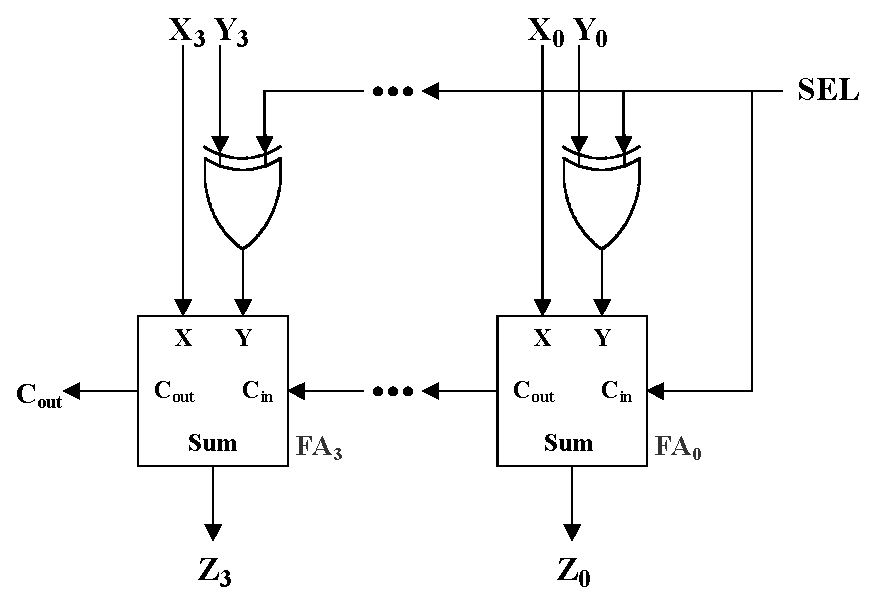
\includegraphics[width=\textwidth]{adder}
%   \caption{\label{fig:adder} 4-bit adder/subtractor.}
% \end{figure}

\begin{table}[hbtp]
  \centering
  \begin{tabular}{c|cc|cc|cc|cc}
 & \multicolumn{2}{c|}{Inputs} & \multicolumn{2}{c|}{PS} & \multicolumn{2}{c|}{NS} & \multicolumn{2}{c}{Outputs} \\
mt & E & U & Q1 & Q0 & Q1+ & Q0+ & Z1 & Z0 \\
\hline
0  & 0 & 0 & 0  & 0  & 1   & 1   & 0  & 0  \\
1  & 0 & 0 & 0  & 1  & 0   & 0   & 0  & 1  \\
2  & 0 & 0 & 1  & 0  & 0   & 1   & 1  & 0  \\
3  & 0 & 0 & 1  & 1  & 1   & 0   & 1  & 1  \\
4  & 0 & 1 & 0  & 0  & 0   & 1   & 0  & 0  \\
5  & 0 & 1 & 0  & 1  & 1   & 0   & 0  & 1  \\
6  & 0 & 1 & 1  & 0  & 1   & 1   & 1  & 0  \\
7  & 0 & 1 & 1  & 1  & 0   & 0   & 1  & 1  \\
8  & 1 & 0 & 0  & 0  & 0   & 0   & 0  & 0  \\
9  & 1 & 0 & 0  & 1  & 0   & 1   & 0  & 1  \\
10 & 1 & 0 & 1  & 0  & 1   & 0   & 1  & 0  \\
11 & 1 & 0 & 1  & 1  & 1   & 1   & 1  & 1  \\
12 & 1 & 1 & 0  & 0  & 0   & 0   & 0  & 0  \\
13 & 1 & 1 & 0  & 1  & 0   & 1   & 0  & 1  \\
14 & 1 & 1 & 1  & 0  & 1   & 0   & 1  & 0  \\
15 & 1 & 1 & 1  & 1  & 1   & 1   & 1  & 1  \\
\end{tabular}
  \caption{\label{tab:values} Transition Table }
\end{table}

$D_1 = Q_1^+ = \sum_m(0,3,5,6,10,11,14,15)$

$D_0 = Q_0^+ = \sum_m(0,2,4,6,9,11,13,15)$

$Q_1^+ = E'U'Q_1'Q_0' + U'Q_1Q_0 + E'UQ_1'Q_0 + UQ_1Q_0' + EQ_1$

$Q_0^+ = E'Q_0' + EQ_0$

% \begin{equation}
%   \label{eq:D1}
%   D_1(E,U,Q_1,Q_0) = Q_1^+ = \sum_m(0,3,5,6,10,11,14,15)
% \end{equation}

% \begin{equation}
%   \label{eq:D2}
%   D_0(E,U,Q_1,Q_0) = Q_0^+ = \sum_m(0,2,4,6,9,11,13,15)
% \end{equation}

% \begin{equation}
%   \label{eq:Q1}
%   Q_1^+ = E'U'Q_1'Q_0' + U'Q_1Q_0 + E'UQ_1'Q_0 + UQ_1Q_0' + EQ_1
% \end{equation}

% \begin{equation}
%   \label{eq:Q0}
%   Q_0^+ = E'Q_0' + EQ_0
% \end{equation}

\section{VHDL}
\label{sec:vhdl}

\begin{verbatim}
library IEEE;
use IEEE.STD_LOGIC_1164.all;

library UNISIM;
use UNISIM.VComponents.all;

use work.project4_pkg.all;

entity counter is
  port (EL  : in  std_logic;  -- Active-low enable
        UP  : in  std_logic;  -- Active-high control (count up/down)
        CLK : in  std_logic;  -- Rising-edge trigger clock
        CLR : in  std_logic;  -- Active-high asynchronous clear
        Z   : out std_logic_vector (1 downto 0));  -- 2-bit number
end counter;

architecture Dataflow of counter is
  signal d        : std_logic_vector(1 downto 0);
  signal q        : std_logic_vector(1 downto 0);
  signal slow_clk : std_logic;

begin
  -- q next-state equations
  d(1) <= (not EL and not UP and not q(1) and not q(0)) or
          (not UP and q(1) and q(0)) or
          (not EL and UP and not q(1) and q(0)) or
          (UP and q(1) and not q(0)) or
          (EL and q(1));
  d(0) <= (not EL and not q(0)) or (EL and q(1));

  -- Stretch the clock input for slow_clk
  CDIV : CLK_DIV port map (CLK, slow_clk);

  -- D flip-flops to do the actual switching
  FF1 : FDC port map(q(1), slow_clk, CLR, d(1));
  FF0 : FDC port map(q(0), slow_clk, CLR, d(0));

  Z <= q;  -- Give Z the present state (for output)
end Dataflow;
\end{verbatim}

\end{document}
